\documentclass[compress]{beamer}
\input{../../resources/preamble.sty}
\addbibresource{../../resources/literature.bib}
\graphicspath{{../../resources/img/}}



\usepackage[utf8]{inputenc}
\usepackage[T1]{fontenc}
\usepackage{lmodern}
\usepackage{tikz}
\usetikzlibrary{positioning,arrows.meta}
\usepackage{graphicx}




\begin{document}

\title[Big Data and Automated Content Analysis]{\textbf{Big Data and Automated Content Analysis (6EC)} 
\\Week 5: »Unsupervised machine learning«
\\Thursday}
\author[Anne Kroon]{Anne Kroon\\ \footnotesize{a.c.kroon@uva.nl \\}}
\date{November 27, 2025}
\institute[UvA CW]{UvA RM Communication Science}


\begin{frame}{}
	\titlepage
\end{frame}

\begin{frame}{Today}
	\tableofcontents
\end{frame}

\question{Everything clear from previous weeks? Questions?}

\begin{frame}[standout]
This week, we will get a general overview of working with textual data. Due to a lack of time, I will introduce you to some of the basic concepts, point you to resources, and give you a practical, hands-on introduction. 
\end{frame}

\begin{frame}{\cite{Boumans2016}: Types of Automated Content Analysis}
	\makebox[\columnwidth]{	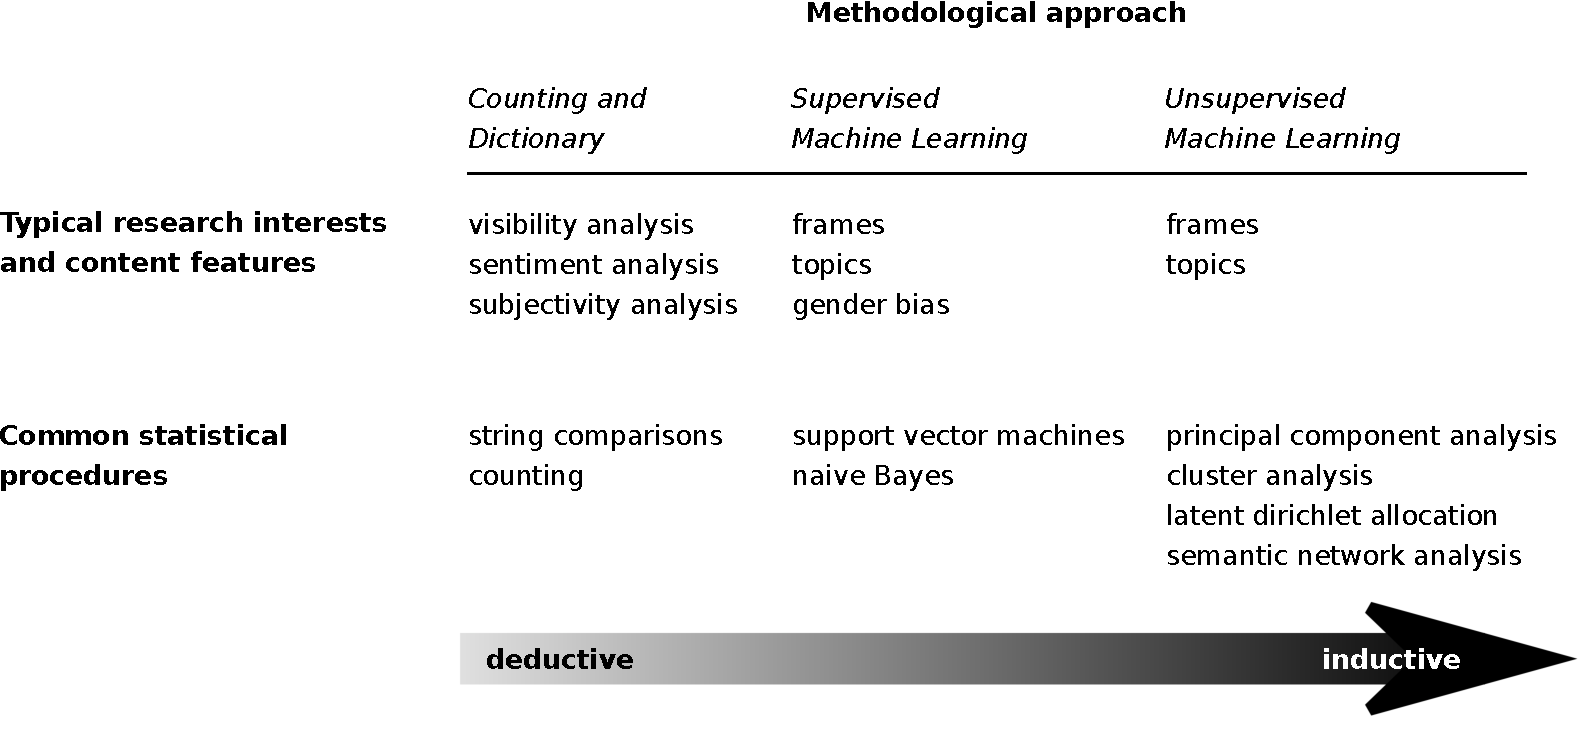
\includegraphics[width=\columnwidth,height=.8\paperheight,keepaspectratio]{boumanstrilling2016}}
\end{frame}

\begin{frame}{Bottom-up vs. top-down}
\begin{block}{Bottom-up}
	\begin{itemize}
		\item Count most frequently occurring words 
		\item Maybe better: Count combinations of words $\Rightarrow$ Which words co-occur together?
	\end{itemize}
	We \emph{don't} specify what to look for in advance	
\end{block}

\onslide<2>{
	\begin{block}{Top-down}
		\begin{itemize}
			\item Count frequencies of pre-defined words
			\item Maybe better: patterns instead of words
		\end{itemize}
		We \emph{do} specify what to look for in advance	
	\end{block}
}

\end{frame}

\begin{frame}[fragile]{A simple bottom-up approach}

\begin{minted}[%
	breaklines,
	linenos,
	fontsize=\scriptsize,
	frame=single,
	xleftmargin=0pt,]
	{python}
from collections import Counter
texts = ["Communication in the Digital Society is a very very complex phenomenon", "I like to study it"]
bottom_up = []
for t in texts:
    bottom_up.append(Counter(t.lower().split()).most_common(3))
    print(bottom_up)
\end{minted}
\pause
This results in:
\begin{minted}[fontsize=\scriptsize]{python}
[('very', 2), ('Communication', 1), ('in', 1)]
[('I', 1), ('like', 1), ('to', 1)]
\end{minted}
\textcolor{red}{\footnotesize{\emph{Please note that you can also write this like:}}}
\pause
\begin{minted}[%
	breaklines,
	linenos,
	fontsize=\scriptsize,
	frame=single,
	xleftmargin=0pt,]
	{python}
bottom_up = [Counter(t.split()).most_common(3) for t  in texts]
\end{minted}
\begin{itemize}
	\tiny{
		\item This is \emph{exactly} the same, just shorter (and faster). 
		\item You do \emph{not} have to use list comprehensions, but it helps if you can read them. }
\end{itemize}

\end{frame}

\begin{frame}[fragile]{A simple top-down approach}
\begin{minted}[%
	breaklines,
	linenos,
	fontsize=\scriptsize,
	frame=single,
	xleftmargin=0pt,]
	{python}
texts = ["Communication in the Digital Society is a very very complex phenomenon", "I like to study it"]
features = ["communication", "digital", "study"]
for t in texts:
    print(f"\nAnalyzing '{t}':")
    for f in features:
        print(f"{f} occurs {t.lower().count(f)} times")
\end{minted}
\pause
\begin{minted}[fontsize=\tiny]{python}
Analyzing 'Communication in the Digital Society is a very very complex phenomenon':
communication occurs 1 times
digital occurs 1 times
study occurs 0 times
	
Analyzing 'I like to study it':
communication occurs 0 times
digital occurs 0 times
study occurs 1 times	
\end{minted}
\end{frame}

\question{When would you use which approach?}

\begin{frame}{Some considerations}
\begin{itemize}[<+->]
	\item Both can have a place in your workflow (e.g., bottom-up as first exploratory step)
	\item You have a clear theoretical expectation? Bottom-up makes little sense.
	\item But in any case: you need to transform your text into something ``countable''.
\end{itemize}
\end{frame}

\section{Unsupervised Machine Learning for Text Classification}


\begin{frame}{Supervised vs Unsupervised}
	\begin{columns}[t]
		\column{.5\textwidth}
		
		\begin{block}<1-4>{Supervised machine learning}
			You have a dataset with both predictor and outcome (independent and dependent variables; features and labels) --- a \emph{labeled} dataset.
			\onslide<2>{
				\footnotesize{Think of regression: You measured \texttt{x1}, \texttt{x2}, \texttt{x3} and you want to predict \texttt{y}, which you also measured}}
		\end{block}
		
		\column{.5\textwidth}
		
		\begin{block}<3->{Unsupervised machine learning}
			You have no labels. \onslide<4>{(\footnotesize{You did not measure \texttt{y})}}\\
			\onslide<5>{\textbf{You might already know \emph{some} techniques to figure out whether \texttt{x1}, \texttt{x2},\ldots \texttt{x\_i} co-occur} \begin{itemize}
					\item Principal Component Analysis (PCA) and Singular Value Decomposition (SVD)
					\item Cluster analysis
					\item Topic modelling (Non-negative matrix factorization and Latent Dirichlet Allocation)
					\item \ldots
			\end{itemize}}
		\end{block}
		
	\end{columns}
	
\end{frame}


\input{../../modules/machinelearning-text/lda.tex}

%================================================
\section{From Bag-of-Words to Embeddings}
%================================================

\begin{frame}{Recap: Document-Term Matrix (DTM)}
    \begin{itemize}
        \item Text is transformed into numerical features:
        \begin{itemize}
            \item raw counts or
            \item TF--IDF values.
        \end{itemize}
        \item Rows = documents, columns = words.
        \item Works well for simple analyses.
    \end{itemize}
\end{frame}

%------------------------------------------------

\begin{frame}{Limitations of Bag-of-Words}
    \begin{itemize}
        \item Treats words as independent features.
        \item Loses context and meaning.
        \item High-dimensional and sparse.
        \item Similar meanings may look unrelated numerically.
        \item Example: ``car'' vs. ``automobile''.
    \end{itemize}
\end{frame}

%------------------------------------------------

\begin{frame}{Motivation: We Want Semantic Similarity}
    \begin{itemize}
        \item Goal in topic modelling:
        \begin{itemize}
            \item Group documents that \textbf{talk about similar things}.
        \end{itemize}
        \item Bag-of-Words relies on exact word overlap.
        \item We want a representation where:
        \begin{itemize}
            \item Similar texts are close together.
            \item Dissimilar texts are far apart.
        \end{itemize}
        \item Enter: \textbf{Embeddings}.
    \end{itemize}
\end{frame}

%================================================
\section{Embeddings}
%================================================

\begin{frame}{What Are Embeddings?}
    \begin{itemize}
        \item Dense numerical vectors representing meaning.
        \item Each document becomes a vector with, e.g., 384 dimensions.
        \item Core idea:
        \begin{block}{Semantic Proximity}
            Documents with similar meaning have similar vectors.
        \end{block}
    \end{itemize}
\end{frame}

%------------------------------------------------

\begin{frame}{Polysemy and Context}
    \begin{itemize}
        \item \textbf{Polysemy}: one word, multiple meanings.
        \item Example: ``bank'' (finance) vs ``bank'' (river).
        \item Bag-of-Words cannot distinguish these.
        \item Embeddings consider context, so the vectors differ.
    \end{itemize}
\end{frame}

%------------------------------------------------

\begin{frame}{Dense vs Sparse Representations}
    \begin{itemize}
        \item Bag-of-Words vectors:
        \begin{itemize}
            \item very high dimensional,
            \item mostly zeros (\textbf{sparse}).
        \end{itemize}
        \item Embeddings:
        \begin{itemize}
            \item low dimensional,
            \item mostly non-zero (\textbf{dense}).
        \end{itemize}
        \item Dense vectors make similarity and clustering easier.
    \end{itemize}
\end{frame}

%------------------------------------------------
% SIMPLE VISUAL

\begin{frame}{From BOW to Embeddings (Visual)}
    \centering
    \begin{tikzpicture}[
        >=Stealth,
        thick,
        block/.style={
            rectangle,
            draw,
            rounded corners,
            minimum width=3.8cm,
            minimum height=1.4cm,
            align=center
        },
        smalltxt/.style={font=\footnotesize}
    ]

    \node[block] (dtm) {
        \textbf{Document-Term Matrix}\\[0.1cm]
        \smalltxt{Counts / TF--IDF\\Sparse, high-dimensional}
    };

    \node[block, right=3.3cm of dtm] (emb) {
        \textbf{Embeddings}\\[0.1cm]
        \smalltxt{Dense vectors\\Meaning-based}
    };

    \draw[->] (dtm) -- node[above, smalltxt]{\textbf{learned mapping}} (emb);

    \node[smalltxt, below=0.4cm of dtm] {
        e.g.\ [0, 0, 3, 0, 1, 0, \dots]
    };
    \node[smalltxt, below=0.4cm of emb] {
        e.g.\ [0.12, -0.48, 0.03, 0.91, \dots]
    };

    \end{tikzpicture}
\end{frame}

%================================================
\section{From Embeddings to BERTopic}
%================================================

\begin{frame}{Why Use Embeddings for Topics?}
    \begin{itemize}
        \item Capture context, synonyms, and meaning.
        \item Similar texts are numerically close.
        \item Better suited for clustering than Bag-of-Words.
        \item Provides a strong basis for modern topic models.
    \end{itemize}
\end{frame}

%------------------------------------------------

\begin{frame}{BERTopic: High-Level Idea}
    \begin{itemize}
        \item Classic models (e.g.\ LDA) use Bag-of-Words.
        \item \textbf{BERTopic} uses embeddings instead.
        \item Then:
        \begin{enumerate}
            \item reduce dimensions,
            \item cluster documents,
            \item extract topic words.
        \end{enumerate}
        \item All steps run automatically in BERTopic.
    \end{itemize}
\end{frame}

%------------------------------------------------
% PIPELINE VISUAL

\begin{frame}{BERTopic Pipeline (Visual Overview)}
    \centering
    \resizebox{\textwidth}{!}{%
    \begin{tikzpicture}[
        >=Stealth,
        thick,
        node distance=1.8cm,
        block/.style={
            rectangle,
            draw,
            rounded corners,
            minimum width=3.0cm,
            minimum height=1.1cm,
            align=center
        },
        smalltxt/.style={font=\footnotesize}
    ]

    \node[block] (docs) {Raw documents};

    \node[block, right=of docs] (emb) {Sentence Transformers\\[0.05cm]
        \smalltxt{document embeddings}};

    \node[block, right=of emb] (umap) {UMAP\\[0.05cm]
        \smalltxt{dimensionality reduction}};

    \node[block, right=of umap] (hdb) {HDBSCAN\\[0.05cm]
        \smalltxt{clusters of documents}};

    \node[block, right=of hdb] (ctfidf) {c-TF--IDF\\[0.05cm]
        \smalltxt{topic words per cluster}};

    \node[block, right=of ctfidf] (topics) {Interpretable topics};

    \draw[->] (docs) -- (emb);
    \draw[->] (emb) -- (umap);
    \draw[->] (umap) -- (hdb);
    \draw[->] (hdb) -- (ctfidf);
    \draw[->] (ctfidf) -- (topics);

    \node[smalltxt, below=0.9cm of hdb, align=center] (outliers)
        {Outliers\\$\Rightarrow$ topic \(-1\)};
    \draw[->] (hdb.south) -- (outliers.north);

    \end{tikzpicture}
    }

    \vspace{0.3cm}
    \small In practice, running \texttt{BERTopic()} executes all steps automatically.
\end{frame}

%------------------------------------------------

\begin{frame}{Key Takeaways}
    \begin{itemize}
        \item Bag-of-Words: counts, sparse, no meaning.
        \item Embeddings: dense vectors encoding semantics.
        \item BERTopic:
        \begin{enumerate}
            \item embeddings,
            \item UMAP,
            \item HDBSCAN,
            \item c-TF--IDF.
        \end{enumerate}
        \item Produces coherent, interpretable topics.
    \end{itemize}
\end{frame}

%------------------------------------------------

\question{Any questions?}

\section{Next steps}

\begin{frame}[standout]

Example notebooks with code for running LDA models and BERTopic models can be found here:
\large{\url{https://github.com/uvacw/teaching-bdaca/blob/main/6ec-course/week05/exercises/}

Note: I would advise to run the BERTopic model on Google Colab so you have access to a GPU. If there is time, we 
can discuss this together in class. }
\end{frame}


\begin{frame}[allowframebreaks,plain]
	\printbibliography
\end{frame}


\section[Appendix]{Appendix: Code examples}


\begin{frame}[fragile,plain]{}
  \begin{minted}{python}
from sklearn import datasets
from sklearn.decomposition import TruncatedSVD
from sklearn.feature_extraction.text import TfidfVectorizer
from sklearn.pipeline import make_pipeline

texts = datasets.fetch_20newsgroups(data_home='rec.autos', remove=('headers', 'footers', 'quotes'), subset='train')['data']

myvec = TfidfVectorizer(max_df=.5, min_df=5, token_pattern='(?u)\\b[a-zA-Z][a-zA-Z]+\\b')
mysvd = TruncatedSVD(n_components=3)
mypipe = make_pipeline(myvec, mysvd)
r = mypipe.fit_transform(texts)
\end{minted}
\end{frame}





\begin{frame}[fragile]{Plotting the texts according to their component scores}
\begin{lstlisting}
import matplotlib.pyplot as plt

fig = plt.figure(figsize=(10,10))
ax = fig.add_subplot(projection='3d')
ax.scatter([e[0] for e in r], [e[1] for e in r],  [e[2] for e in r],alpha=.2)
\end{lstlisting}

\makebox[\linewidth]{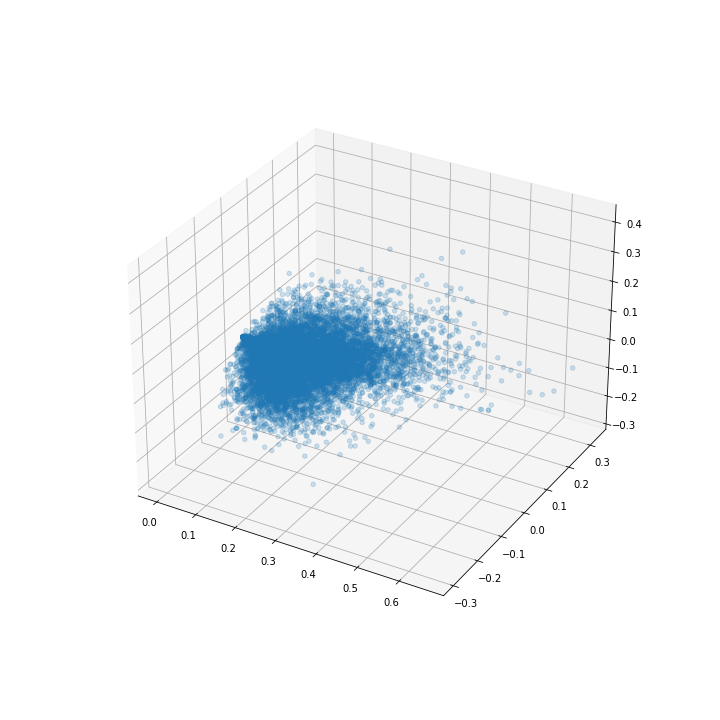
\includegraphics[width=\paperwidth,height=.6\paperheight,keepaspectratio]{svd3d}}

\end{frame}



\begin{frame}[fragile]{Using the scores}
\begin{lstlisting}
import pandas as pd
textscores= pd.DataFrame(r)
featurescores = pd.DataFrame(mysvd.components_.T, index = myvec.get_feature_names())
\end{lstlisting}

\makebox[\linewidth]{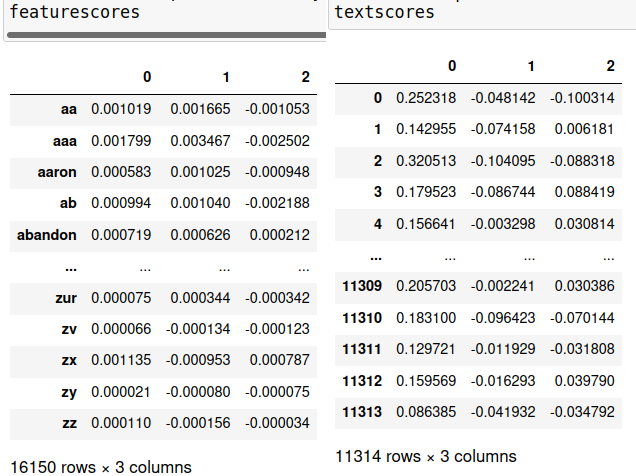
\includegraphics[width=\paperwidth,height=.6\paperheight,keepaspectratio]{svdscores}}

\end{frame}



\begin{frame}{Grouping features vs grouping cases}
  We have a  corpus of a many texts.
  
\begin{itemize}
\item We used SVD to figure out relationships between features
\item We could now look at the most important features per component (``topic'', ``frame''?) by sorting \texttt{featurescores}
\item We could see which texts are most representative for each ``topic'' or ``frame'' by sorting \texttt{textscores}
\end{itemize}
\pause

$\Rightarrow$ Alternative: Choose the opposite approach and first find out which cases are most similar, \textit{then} describe what features characterize each group of cases


\end{frame}


\begin{frame}[plain,fragile]
\begin{minted}{python}
from sklearn.cluster import KMeans

k = 5

mykm = KMeans(n_clusters=k, init='k-means++', max_iter=100, n_init=1)
myvec = TfidfVectorizer(max_df=.5, min_df=5, token_pattern='(?u)\\b[a-zA-Z][a-zA-Z]+\\b')
mypipe = make_pipeline(myvec, mykm)

predictions = mypipe.fit_transform(texts)
# potentially: textscores = pd.Dataframe(predictions)
\end{minted}

Of course, you need to determine the appropriate $k$\ldots (see earlier lecture)



\end{frame}


\begin{frame}[fragile,plain]{Let's get the terms closest to the centroids}
\begin{lstlisting}
order_centroids = mykm.cluster_centers_.argsort()[:, ::-1]
terms = myvec.get_feature_names()

print("Top terms per cluster:")

for i in range(k):
    print("Cluster {}: ".format(i), end='')
    for ind in order_centroids[i, :10]:
        print("{} ".format(terms[ind]), end='')
    print()

\end{lstlisting}
\pause
returns something like:

\begin{lstlisting}
Top terms per cluster:
Cluster 0: windows file dos window with on you this have files 
Cluster 1: you on this was with are have be not they 
Cluster 2: thanks any me have anyone or please if on this 
Cluster 3: he was his him not as this but on god 
Cluster 4: you are be not they as this have if on 
\end{lstlisting}
(of course, we could do sth similar with pandas as well)
\end{frame}



\end{document}
